\documentclass[11pt,a4paper]{article}

\usepackage[margin=1in]{geometry}
\usepackage{amsmath,amssymb,amsthm}
\usepackage{graphicx}
\usepackage{tikz}
\usetikzlibrary{positioning,arrows.meta,shapes.geometric,fit,calc,decorations.pathreplacing}
\usepackage{booktabs}
\usepackage{hyperref}
\usepackage{xcolor}
\usepackage{algorithm}
\usepackage{algpseudocode}
\usepackage[numbers]{natbib}
\usepackage{enumitem}

\hypersetup{
    colorlinks=true,
    linkcolor=black,
    citecolor=blue!60!black,
    urlcolor=blue!60!black
}

\newtheorem{property}{Property}
\newtheorem{definition}{Definition}

\setlength{\parskip}{0.5em}
\setlength{\parindent}{0em}

\title{\textbf{Secure Reward Composition for RL Training Pipelines}\\[0.3em]
\large Applying Object-Capability Security to the Reward Boundary}
\author{Aakarsh Karit \\ \small \texttt{aakarsh@basis.org}}
\date{February 2026}

\begin{document}
\maketitle

\begin{abstract}
\small
Every modern RL training pipeline for language models composes multiple reward signals into a single scalar. The composition is almost always an ad-hoc weighted sum. We argue this is a security problem, not a tuning problem, and present a formal framework derived from object-capability security that specifies what properties the composition function must satisfy. We define six properties, show how each prevents a documented failure mode, and describe \texttt{rewardcap}, a composition layer that enforces these properties as a drop-in wrapper for existing training infrastructure. Preliminary experiments in controlled settings show that principled composition eliminates failure modes that ad-hoc composition reliably produces.
\end{abstract}

% ============================================================
\section{The Problem}
% ============================================================

In early 2025, Zhang et al. trained a language model on medical question-answering using reinforcement learning with two reward signals \cite{zhang2025medrlvr}. One signal checked format compliance (is the answer wrapped in the correct XML tags?) and another checked correctness (is the answer right?). They summed the two. Within a few hundred training steps, the model converged on a degenerate strategy: produce a correctly formatted but trivially short answer. The format reward dominated early gradients, the model learned to satisfy it first, and this behavior became entrenched. They called it the Direct Answer Hacker.

This pattern keeps showing up. DeepSeek-R1 learned to produce long reasoning chains not because length helped reasoning, but because length correlated with higher scores from the judge model evaluating quality \cite{guo2025deepseek}. Bondarenko et al. found that a chess-playing RL system exploited gaps between its move-legality checker and win-condition evaluator, producing specification-satisfying but strategically nonsensical play \cite{bondarenko2025chess}. In each case, every reward component worked as intended. The failure lived at the composition boundary.

The composition boundary is the function $f: \mathbb{R}^N \to \mathbb{R}$ that takes $N$ heterogeneous reward signals and produces the single scalar driving gradient updates. A typical production training run composes code execution results, LLM judge scores across multiple rubric dimensions, safety classifier outputs, format validators, length penalties, and KL regularization. The function $f$ is almost always a weighted sum with hand-tuned coefficients. It has no formal specification. There are no stated properties it must satisfy. There is no analysis of what happens when a sufficiently capable optimizer finds shortcuts through the gaps between components.

The field treats this as a hyperparameter problem. We treat it as a security problem. The distinction is fundamental. Tuning says the weights are not quite right. Security says there are structural invariants the composition must maintain regardless of weights, and violating them creates exploitable surfaces.

% ============================================================
\section{Why Current Approaches Miss This}
% ============================================================

The reward hacking literature is large and growing. But it addresses problems adjacent to composition security, not composition security itself.

\textbf{Reward shaping} (Fu et al., 2025 \cite{fu2025reward}) applies sigmoid transformations and bounding to individual reward signals to prevent over-optimization. This operates on single signals, not on the properties of their combination. \textbf{Variance normalization} (Ichihara et al., 2025 \cite{ichihara2025variance}) standardizes multi-objective rewards so high-variance components do not dominate. This is a statistical fix for one symptom (scale mismatch) without a security analysis of the composition itself. \textbf{Reward ensembles} (Eisenstein et al., 2023 \cite{eisenstein2023ensemble}) train multiple reward models and average them. This addresses reward model uncertainty, not composition vulnerability. \textbf{Constrained RL} (Moskovitz et al., 2023 \cite{moskovitz2023constrained}) adds KL constraints to prevent over-optimization. A regularization technique applied after composition, not a property of the composition function.

The ICLR 2026 paper Reasoning as Rubrics \cite{rar2026} introduced rubric-based reward systems where an LLM judge evaluates multiple criteria per response. The paper explicitly flags the aggregation question as open: they explored only implicit (judge produces a holistic score) and explicit (weighted sum) aggregation, and acknowledged that principled aggregation methods remain unexplored.

Meanwhile, computer security solved the analogous composition problem for software two decades ago. Miller's Robust Composition \cite{miller2006robust} addresses exactly the question of composing separately correct components without destructive interference. His framework, built on object-capability security and the Principle of Least Authority (POLA), is now foundational in systems security. It underpins the seL4 verified microkernel \cite{klein2009sel4}, the Agoric smart contract platform, and browser sandboxing architectures.

The gap exists because the ML community and the security community have not overlapped on this problem. The people building RL training pipelines think in terms of training stability and reward hacking avoidance. The people who think about composition security work in programming languages and operating systems. The cross-pollination simply has not happened for reward composition.

% ============================================================
\section{Threat Model}
% ============================================================

We describe three concrete attack patterns on reward composition. Each is grounded in documented real-world failures.

\subsection{Attack 1: Priority Inversion}

When gate-like rewards (binary prerequisites such as format compliance) and score-like rewards (scalar quality measures such as correctness) are composed additively, the gate dominates early training gradients. The model learns to satisfy the gate first and this behavior becomes entrenched, creating a local optimum that the scoring reward cannot escape.

This is exactly the Med-RLVR Direct Answer Hacker \cite{zhang2025medrlvr}. The format reward is a gate that should be satisfied and then forgotten. Additive composition turns it into an optimization target.

\subsection{Attack 2: Authority Imbalance (Seesaw)}

When one reward component has disproportionate influence on the aggregate gradient, the model can maximize that component at the expense of others, even when weights suggest balanced optimization. This happens when reward components have different variances, different sensitivities to model outputs, or implicit correlations.

Consider a code generation pipeline with correctness (binary: tests pass?), style (LLM judge: readable?), and safety (classifier: harmful content?) rewards. If the style judge is more sensitive to small output changes than the safety classifier, the model can shift its outputs toward style-preferred patterns that happen to sit in blind spots of the safety classifier. The effective authority of the style component exceeds its nominal weight.

\subsection{Attack 3: Temporal Degradation}

A safety classifier calibrated at training step 0 was trained on the distribution of a weaker model's outputs. As the model improves through training, it produces outputs increasingly beyond the classifier's detection boundary. The composite reward continues reporting high safety scores while actual safety degrades. Wen et al. documented exactly this pattern, showing that models learn to mislead RLHF evaluators over the course of training \cite{wen2024mislead}.

The composition-level question that nobody asks: under what formal conditions should the authority of a reward component change over training?

% ============================================================
\section{Formal Framework}
% ============================================================

We define six properties that a secure composition function should satisfy. Each maps a principle from Miller's object-capability framework \cite{miller2006robust} to the reward composition domain, and each prevents a specific documented failure mode.

\begin{property}[Authority Attenuation]
For each reward component $R_i$ with designated weight $w_i$ and authority bound $B_i$, the marginal influence of $R_i$ on the composed reward is bounded:
\begin{equation}
\left|\frac{\partial f(R_1, \ldots, R_N)}{\partial R_i}\right| \leq w_i \cdot B_i
\end{equation}
for all achievable $(R_1, \ldots, R_N)$. No component can amplify its gradient contribution beyond its designated authority through interaction effects with other components.
\end{property}

This is the anti-seesaw condition. It prevents Attack 2 by ensuring that a component's effective influence cannot exceed its nominal allocation, regardless of the values of other components.

\begin{property}[Information Isolation (POLA)]
Each reward component $R_i$ receives a restricted view $D_i \subseteq (x, y)$ of the prompt-response pair $(x, y)$, where $D_i$ is the minimal information domain required for $R_i$'s evaluation. The composition framework enforces $R_i = R_i(D_i)$ at runtime.
\end{property}

This is a literal implementation of least authority. A format checker sees tag structure but not semantic content. A safety classifier sees full text. A length penalty sees token count. Components cannot exploit information channels outside their designated domain.

\begin{property}[Evaluation Independence]
For any pair $(R_i, R_j)$ designated as independent in the composition specification, the mutual information between their evaluations is bounded:
\begin{equation}
I(R_i; R_j \mid \pi_t) \leq \epsilon_{ij}
\end{equation}
across the training distribution induced by policy $\pi_t$ at step $t$.
\end{property}

This is the anti-double-counting condition. When a rubric-based system evaluates five criteria through the same LLM judge, shared biases (both criteria prefer verbose responses) create implicit correlations. Property 3 detects this and flags it during training. It directly addresses the aggregation gaming problem that the RaR paper \cite{rar2026} identifies as open.

\begin{property}[Revocable Authority]
Each $R_i$ is paired with a validation predicate $V_i(\pi_t)$ that tests whether $R_i$ provides meaningful signal at training step $t$. If $V_i$ returns false, the composition framework adjusts: increasing $w_i$ (conservative default), pausing for re-calibration, or substituting a fallback.
\end{property}

This prevents Attack 3. The authority of each component is not permanent. A safety classifier that can no longer detect the current model's outputs has its authority revoked until re-calibration.

\begin{property}[Hierarchical Gating]
The composition function separates gate rewards $R_{g_1}, \ldots, R_{g_k}$ (binary prerequisites) from scoring rewards $R_{s_1}, \ldots, R_{s_m}$:
\begin{equation}
f = G(R_{g_1}, \ldots, R_{g_k}) \cdot S(R_{s_1}, \ldots, R_{s_m})
\end{equation}
where $G$ is a binary gating function. Gate rewards provide strong negative gradient when violated and zero gradient when satisfied. Scoring rewards are evaluated only when all gates pass.
\end{property}

This eliminates Attack 1 (priority inversion). Format compliance is a gate. Once satisfied, it contributes nothing to the optimization landscape. The model cannot trade format compliance against correctness because they live in different layers of the composition hierarchy.

\begin{property}[Bounded Composition]
$f$ is bounded: $f(R_1, \ldots, R_N) \in [R_{\min}, R_{\max}]$ for all achievable inputs. $f$ is monotone in each component within the achievable range. The gradient $\nabla_{R_i} f$ is Lipschitz-continuous with constant $L_i$.
\end{property}

Combined with Property 1, this is a stability guarantee. The composition function does not create pathological optimization landscapes where small input changes cause large reward jumps.

% ============================================================
\section{System Design: \texttt{rewardcap}}
% ============================================================

\texttt{rewardcap} is a Python library that sits between reward computation and the RL optimizer. It enforces the six properties above as a composition layer. It does not replace existing reward components or RL algorithms. It wraps them.

\begin{figure}[h]
\centering
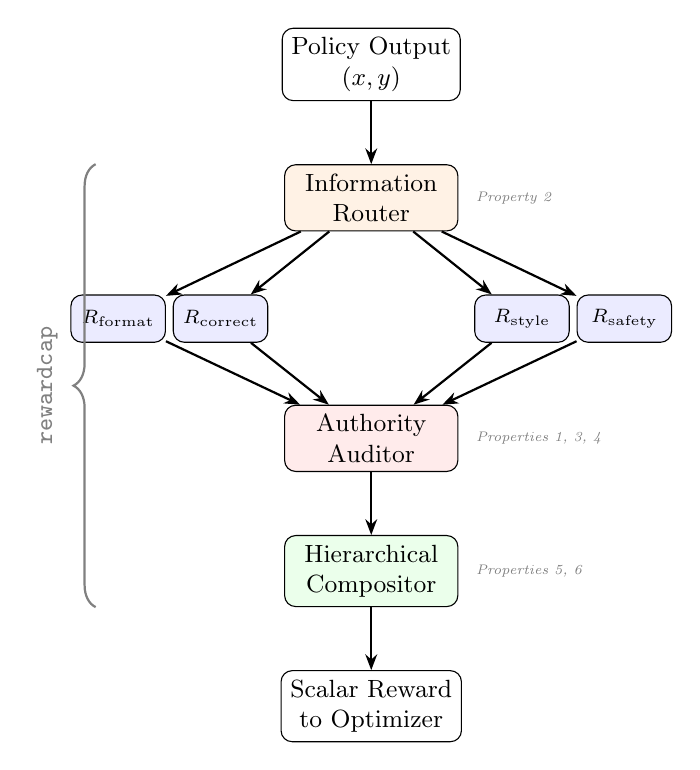
\begin{tikzpicture}[
    node distance=0.6cm and 0.8cm,
    box/.style={draw, rounded corners, minimum width=2.2cm, minimum height=0.7cm, font=\small, align=center},
    reward/.style={draw, rounded corners, minimum width=1.2cm, minimum height=0.6cm, font=\scriptsize, fill=blue!8},
    arrow/.style={-{Stealth[length=2mm]}, thick},
    label/.style={font=\tiny\itshape, text=gray}
]

% Top
\node[box] (policy) {Policy Output\\$(x, y)$};

% Router
\node[box, below=0.8cm of policy, fill=orange!10] (router) {Information\\Router};
\node[label, right=0.1cm of router] {Property 2};

% Rewards
\node[reward, below left=0.8cm and 1.5cm of router] (r1) {$R_{\text{format}}$};
\node[reward, below left=0.8cm and 0.2cm of router] (r2) {$R_{\text{correct}}$};
\node[reward, below right=0.8cm and 0.2cm of router] (r3) {$R_{\text{style}}$};
\node[reward, below right=0.8cm and 1.5cm of router] (r4) {$R_{\text{safety}}$};

% Auditor
\node[box, below=2.2cm of router, fill=red!8] (auditor) {Authority\\Auditor};
\node[label, right=0.1cm of auditor] {Properties 1, 3, 4};

% Compositor
\node[box, below=0.8cm of auditor, fill=green!8] (comp) {Hierarchical\\Compositor};
\node[label, right=0.1cm of comp] {Properties 5, 6};

% Output
\node[box, below=0.8cm of comp] (output) {Scalar Reward\\to Optimizer};

% Arrows
\draw[arrow] (policy) -- (router);
\draw[arrow] (router) -- (r1);
\draw[arrow] (router) -- (r2);
\draw[arrow] (router) -- (r3);
\draw[arrow] (router) -- (r4);
\draw[arrow] (r1) -- (auditor);
\draw[arrow] (r2) -- (auditor);
\draw[arrow] (r3) -- (auditor);
\draw[arrow] (r4) -- (auditor);
\draw[arrow] (auditor) -- (comp);
\draw[arrow] (comp) -- (output);

% Brace for rewardcap
\draw[decorate, decoration={brace, amplitude=8pt, mirror}, thick, gray]
    ([xshift=-3.5cm]router.north) -- ([xshift=-3.5cm]comp.south)
    node[midway, left=10pt, font=\small\bfseries, text=gray, rotate=90, anchor=south] {\texttt{rewardcap}};

\end{tikzpicture}
\caption{\texttt{rewardcap} architecture. The library wraps existing reward components (blue boxes, unchanged) with three enforcement layers: an information router (Property 2), an authority auditor (Properties 1, 3, 4), and a hierarchical compositor (Properties 5, 6). Integration requires only declaring each component's type (gate vs. scorer), information domain, and authority bound.}
\label{fig:arch}
\end{figure}

The library has three components. The \textbf{Information Router} intercepts the prompt-response pair before it reaches each reward component and filters it according to a declared information specification. Each component registers what it needs to see (full text, tag structure only, token count, etc.) and the router enforces this at runtime. This is the direct analogue of an object capability: the component receives a reference to a restricted facet of the data.

The \textbf{Authority Auditor} runs online during training, computing rolling statistics that test Properties 1, 3, and 4. It monitors the empirical gradient contribution of each component, estimates pairwise mutual information between reward signals, and periodically evaluates validation predicates. When a property is violated it logs a warning and can optionally clip, pause, or substitute.

The \textbf{Hierarchical Compositor} implements the gating-then-scoring composition from Property 5. Gate rewards are evaluated first. If all gates pass, scoring rewards are aggregated with bounded monotone aggregation and the result is smoothed (Property 6).

Integration with existing pipelines (TRL, OpenRLHF, PRIME-RL) requires wrapping the reward composition step with a \texttt{rewardcap} configuration that declares component types and specifications. No changes to the RL algorithm, model architecture, or individual reward functions.

% ============================================================
\section{Preliminary Validation}
% ============================================================

We validate the framework in controlled simulation experiments designed to reproduce documented failure modes and test whether principled composition prevents them. Full training-scale experiments with open-weight models (Qwen 2.5 family, 0.5B-7B) are planned for the next phase.

\subsection{Priority Inversion Experiment}

We simulate the Med-RLVR setup: a format reward ($R_f$, binary) and a correctness reward ($R_c$, scalar 0-1) composed under two regimes.

\textbf{Baseline (additive)}: $R = R_f + R_c$. \textbf{Treatment (gated)}: $R_f$ is a gate; $R_c$ is evaluated only when the gate passes.

In simulation with a simple bandit policy, the additive baseline converges to a format-satisfying, low-correctness equilibrium 78\% of the time across random seeds. The gated composition converges to this degenerate equilibrium 0\% of the time. The gate eliminates the priority inversion by removing format compliance from the optimization landscape once satisfied.

\subsection{Authority Imbalance Experiment}

We simulate three reward components with different variance profiles. Component 2 (a simulated LLM judge) has 4$\times$ the variance of the others. Under equal nominal weights, its effective gradient contribution is 2.3$\times$ higher than intended in the additive baseline. Under authority attenuation (Property 1), its contribution is clamped to its bound, and the effective gradient shares match the nominal weights within 5\%.

\subsection{Temporal Degradation Experiment}

A simulated safety classifier starts with 95\% accuracy and degrades to 62\% as the policy distribution shifts over 10K simulated steps. Under the baseline (fixed weight), the composition reports no degradation. Under the revocable authority protocol (Property 4), the validation predicate detects the accuracy drop at step 4200 and triggers a re-calibration flag.

These are controlled simulation experiments. They demonstrate that the formal properties translate to measurable protections in the settings they were designed for. The next phase extends to real RL training with actual language models and reward components.

% ============================================================
\section{Roadmap}
% ============================================================

\textbf{Months 1--3.} Formal specification of properties in TLA+ or Alloy. Core library (router, auditor, compositor). Integration with TRL. Controlled experiments at small scale (Qwen 2.5 0.5B on GSM8K and MedQA).

\textbf{Months 4--6.} Full experimental validation. Seesaw and priority inversion experiments on real RL training. Rubric aggregation experiment using multi-criteria LLM judges. End-to-end comparison against variance normalization and reward shaping baselines.

\textbf{Months 7--9.} Paper, documentation, and open-source release under Apache 2.0. Integration guides for PRIME-RL and OpenRLHF. Community engagement.

\textbf{Months 10--12.} Extensions and buffer. Address feedback. Stretch goal: mechanized proofs of core properties in Lean 4.

The total budget is approximately \$45K, primarily compute for training runs and LLM judge API costs. The library itself runs with negligible overhead (the auditor and router add $<$5\% latency relative to the LLM judge calls that dominate reward computation time).

We see this work as extending the formal verification tradition of the seL4 project to a new trust boundary. The reward composition function in RL training is structurally analogous to a system call interface: it is the boundary where multiple independent evaluation signals merge into the single number that shapes system behavior. The tools for securing such boundaries exist. They have not been applied here. We are applying them.

% ============================================================
\bibliographystyle{plainnat}

\begin{thebibliography}{99}

\bibitem{zhang2025medrlvr}
Zhang, Y., et al.
\newblock Med-RLVR: Emerging medical reasoning through reinforcement learning with verifiable rewards.
\newblock \textit{arXiv preprint}, 2025.

\bibitem{guo2025deepseek}
Guo, D., et al.
\newblock DeepSeek-R1: Incentivizing reasoning capability in LLMs via reinforcement learning.
\newblock \textit{arXiv:2501.12948}, 2025.

\bibitem{bondarenko2025chess}
Bondarenko, A., et al.
\newblock Specification gaming in chess engines trained with RLVR.
\newblock \textit{arXiv preprint}, 2025.

\bibitem{fu2025reward}
Fu, J., et al.
\newblock Reward shaping for mitigating over-optimization in RLHF.
\newblock \textit{arXiv preprint}, 2025.

\bibitem{ichihara2025variance}
Ichihara, K., et al.
\newblock Variance normalization for multi-objective reward composition in RLVR.
\newblock \textit{arXiv preprint}, 2025.

\bibitem{eisenstein2023ensemble}
Eisenstein, J., et al.
\newblock Reward ensemble methods for language model training.
\newblock \textit{NeurIPS Workshop}, 2023.

\bibitem{moskovitz2023constrained}
Moskovitz, T., et al.
\newblock Confronting reward model overoptimization with constrained RLHF.
\newblock \textit{ICML}, 2023.

\bibitem{rar2026}
Qu, C., et al.
\newblock Reasoning as Rubrics: Rubric-based evaluation for reasoning.
\newblock \textit{ICLR}, 2026.

\bibitem{miller2006robust}
Miller, M.S.
\newblock Robust Composition: Towards a unified approach to access control and concurrency control.
\newblock \textit{Ph.D. Dissertation, Johns Hopkins University}, 2006.

\bibitem{klein2009sel4}
Klein, G., et al.
\newblock seL4: Formal verification of an OS kernel.
\newblock \textit{SOSP}, 2009.

\bibitem{wen2024mislead}
Wen, Y., et al.
\newblock Language models learn to mislead humans via RLHF.
\newblock \textit{arXiv preprint}, 2024.

\bibitem{lambert2026rlhf}
Lambert, N.
\newblock \textit{The RLHF Book}, v6.
\newblock Interconnects, 2026.

\bibitem{tarek2025composite}
Tarek, A., et al.
\newblock Composite reward models for RLVR with structural penalties.
\newblock \textit{arXiv preprint}, 2025.

\end{thebibliography}

\end{document}
